\subsection{Schedule}
Until we get the schedule for next semester with more specific dates, we are only able to identify some key phases and tasks that we will need to complete, but we cannot attach them to dates. Additionally, as we work more on development, this schedule may change as we face challenges, or finish tasks quicker than we estimated. Our current schedule overview and plan is as follows:\begin{description}
\item[January –- February]Work with Teams\begin{itemize}
	\item Rebaseline prototype, prioritize requirements
	\item Plan for CS477b specifics, including transition strategy
	\item Participate in ARB review
\end{itemize}
\item[February –- May]Scheduled Weekly Meetings to:\begin{itemize}
	\item Discuss status and plans
	\item Provide access to key transition people for strategy and readiness discussions 
\end{itemize}
\item[March 3--7]Iteration Assessment Reviews
\item[March 26]Core Capability Drivethrough
\item[April 14--18]Project Transition Readiness ARB Reviews
\item[April 21]Installation and Transition\begin{itemize}
	\item Install Product
	\item Execute Transition Plan
\end{itemize}
\item[April 28]Operational Commitment Review for Initial Operational Capability
\item[May 5]Client Evaluations
\end{description}

\clearpage

\subsection{Project}
We have created a project using Microsoft Project to track tasks, phases, and progress. These will be drastically updated as we are provided a more specific schedule of requirements, however sample charts can be seen below.
\begin{figure}[!htbp]
\centering
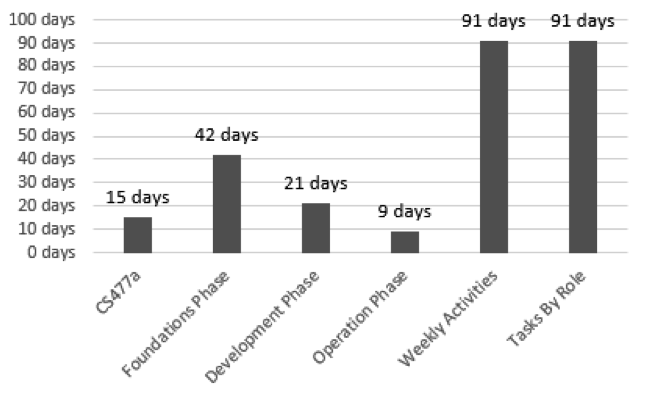
\includegraphics[scale=0.7]{images/completeness.png}
\end{figure}
\begin{figure}[!htbp]
\centering
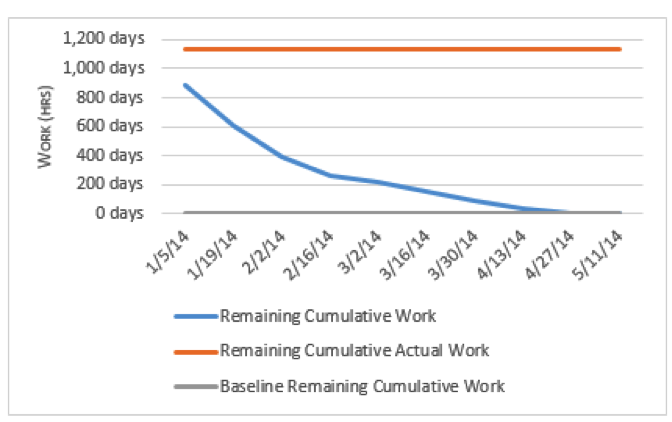
\includegraphics[scale=0.7]{images/graph.png}
\end{figure}

\clearpage

\subsection{Phases and Milestones}
Phases planned in the second semester include the end of the Foundations Phase, the Development Phase, which has two parts, construction and transition, and the Operations Phase. 
Milestones include the RDCR (Rebaselined Development Commitment Review), CCD (Core Capability Drivethrough), TRR (Transition Readiness Review) and OCR (Operational Commitment Review). 
Our tentative schedule of necessary phases and milestones is below:

\begin{figure}[!htbp]
\centering
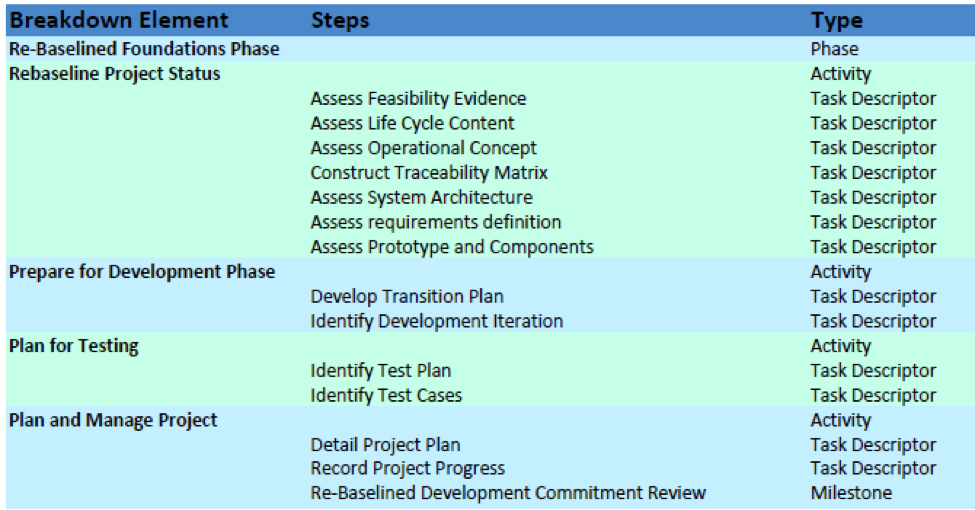
\includegraphics[scale=0.5]{images/table1.png}
\end{figure}
\begin{figure}[!htbp]
\centering
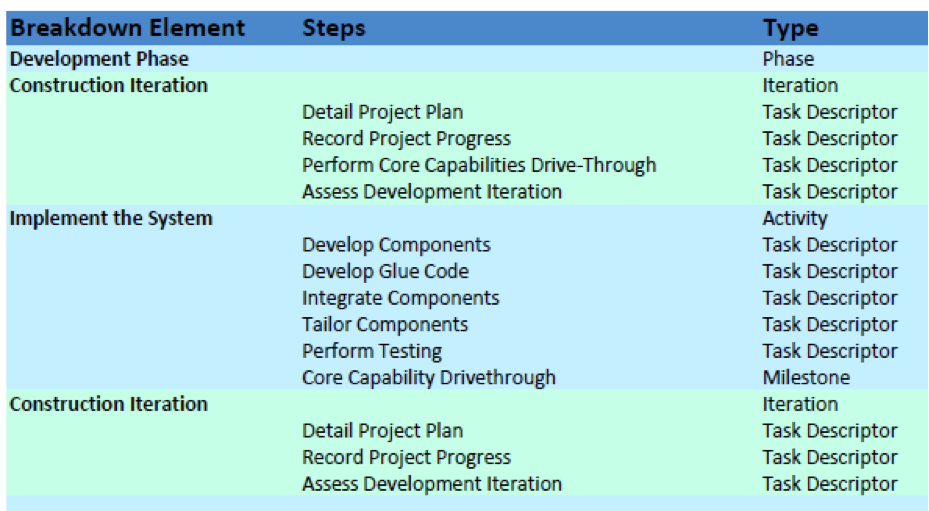
\includegraphics[scale=0.5]{images/table2.png}
\end{figure}
\begin{figure}[!htbp]
\centering
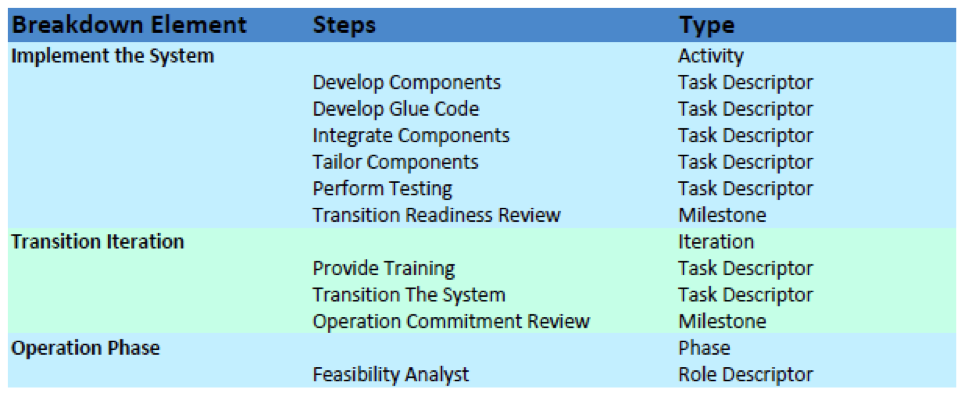
\includegraphics[scale=0.5]{images/table3.png}
\end{figure}

\subsection{Team}
For our team structure and roles, we will have each member coding, testing, and reviewing the work of someone else on the team. We plan to have peer coding, where two people code together. While each member will be have multiple roles and responsibilities, we have broken the team up into front-end and back-end, testers and trainers, and then each member will be an implementer. As the semester of 477b progresses, we may update these roles as we feel necessary, depending on how we progress. 
The following charts lists the team structure and each team member, their positions for 477a/b, and their tentative roles and responsibilities. As we begin work, these may change due to what the team needs.

\begin{figure}[!htbp]
\centering
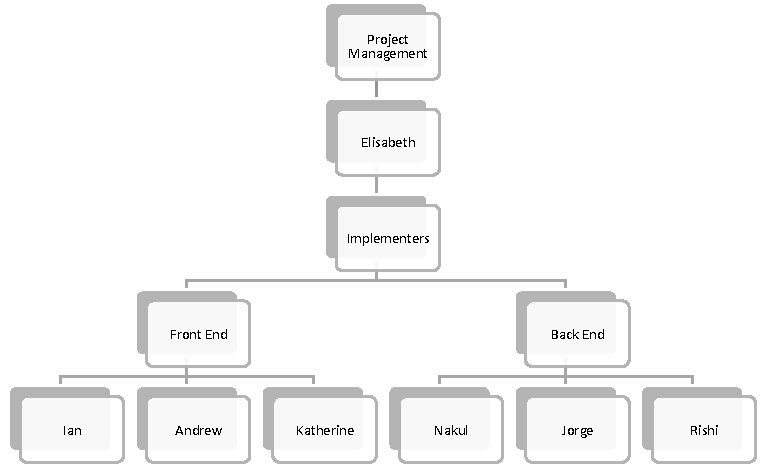
\includegraphics[width=0.7\textwidth]{images/implementation.pdf}
\caption{Team Structure: Implementation}
\end{figure}

\begin{figure}[!htbp]
\centering
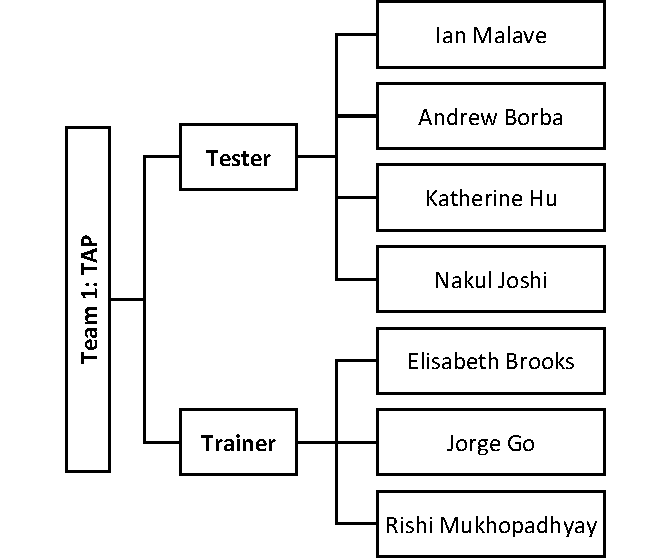
\includegraphics[width=0.7\textwidth]{images/testingtraining.pdf}
\caption{Team Roles: Testing and Training}
\end{figure}

\clearpage

% Please remember to add \use{multirow} to your document preamble in order to suppor multirow cells
% Booktabs require to add \usepackage{booktabs} to your document preamble
\begin{table}[h]
\begin{tabularx}{\textwidth}{@{}llX@{}}
\toprule
Team Member                                                 & Role                          & Responsibility                                               \\ \midrule
Elisabeth Brooks                                            & Project Manager               & Create and manage schedules                                  \\
                                                            &                               & Maintain project management tool (Asana)                     \\
                                                            &                               & Hold team members accountable                                \\
Ian Malave                                                  & Requirements Engineer         & Develop front-end and prototype                              \\
                                                            & Front End Developer           & Update requirements to match prototype                       \\
Andrew Borba                                                & Prototyper                    & Create application prototypes                                \\
                                                            & Front End Developer           & Develop the front-end                                        \\
Katherine Hu                                                & Life Cycle Planner            & Validate application design                                  \\
                                                            & Front End Developer           & Ensure user-friendliness and legibility                      \\
Nakul Joshi                                                 & Systems Architect             & System \& security design on high-level back-end development \\
                                                            & Back End Developer            & Manage LaTeX documentation                                   \\
Jorge Go                                                    & Feasibility Analyst           & Identify and analyze risks                                   \\
                                                            & Back End Developer            & Plan risk mitigation strategies                              \\
                                                            &                               & Run business case and cost-benefit analysis                  \\
Rishi & Operational Concept & Implement back-end                                           \\
Mukhopadyay                                                        & Engineer           & Plan database structure              \\
& Back End Developer &                       

\\ \bottomrule
\end{tabularx}
\end{table}